\documentclass[tikz,border=0pt]{standalone}
\usepackage[T1]{fontenc}
\usepackage{lmodern}
\usepackage{amssymb}
\usetikzlibrary{arrows.meta}
% Generated from reproduction/scope.json. Do not edit by hand.
\newcommand{\SolanaCore}{832{,}941}
\newcommand{\SolanaLifecycle}{1{,}651}
\newcommand{\BaseCore}{62{,}618}
\newcommand{\BaseLifecycle}{62{,}618}
\newcommand{\BNBCore}{1{,}593{,}679}
\newcommand{\BNBLifecycle}{15{,}403}
\newcommand{\TronCore}{104{,}548}
\newcommand{\TronLifecycle}{1{,}831}


\definecolor{Ink}{HTML}{18324A}
\definecolor{Muted}{HTML}{607286}
\definecolor{Divider}{HTML}{CBD5E1}
\definecolor{Surface}{HTML}{F7F9FC}
\definecolor{Blue}{HTML}{184D77}
\definecolor{LightBlue}{HTML}{EAF1F7}
\definecolor{Teal}{HTML}{128078}
\definecolor{LightTeal}{HTML}{E7F3F1}
\definecolor{Purple}{HTML}{7251B5}
\definecolor{LightPurple}{HTML}{F0EBF7}
\definecolor{Amber}{HTML}{B87813}
\definecolor{LightAmber}{HTML}{FFF4DC}
\definecolor{Green}{HTML}{257F55}
\definecolor{LightGreen}{HTML}{E8F4EE}
\definecolor{Red}{HTML}{AA3730}
\definecolor{LightRed}{HTML}{FBECEA}

\newcommand{\BodyFont}{\sffamily\fontsize{8}{8.4}\selectfont}
\newcommand{\TitleFont}{\sffamily\bfseries\fontsize{9.2}{10.2}\selectfont}
\newcommand{\PanelFont}{\sffamily\bfseries\fontsize{8.4}{9.2}\selectfont}

\tikzset{
  panel/.style={rounded corners=2.2pt, draw=Divider, line width=0.55pt, fill=white},
  pill/.style={rounded corners=1.5pt, draw=Divider, line width=0.45pt, fill=white,
    inner xsep=2.2pt, inner ysep=1.5pt, font=\BodyFont, text=Ink},
  flow/.style={-{Latex[length=2.3mm,width=1.5mm]}, draw=Ink, line width=0.75pt},
  body/.style={font=\BodyFont, text=Ink, align=left},
}

\begin{document}
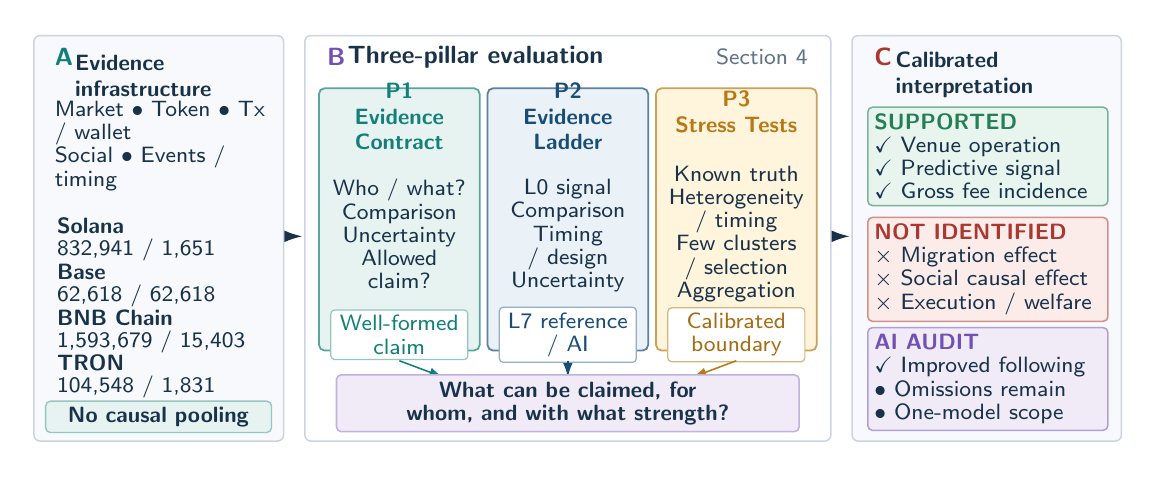
\begin{tikzpicture}[x=1cm,y=1cm]
  \path[use as bounding box] (0,0) rectangle (13.97,5.35);
  \fill[white] (0,0) rectangle (13.97,5.35);

  \draw[panel, fill=Surface] (0.08,0.10) rectangle (3.25,5.25);
  \draw[panel] (3.52,0.10) rectangle (10.20,5.25);
  \draw[panel, fill=Surface] (10.47,0.10) rectangle (13.89,5.25);
  \draw[flow] (3.27,2.70) -- (3.49,2.70);
  \draw[flow] (10.22,2.70) -- (10.44,2.70);

  % A. Evidence infrastructure.
  \node[anchor=west, font=\TitleFont, text=Teal] at (0.22,4.98) {A};
  \node[anchor=north west, font=\PanelFont, text=Ink, align=left] at (0.48,5.12) {Evidence\\infrastructure};
  \node[body, anchor=west, text width=2.72cm] at (0.22,3.85) {Market $\bullet$ Token $\bullet$ Tx / wallet\\Social $\bullet$ Events / timing};

  \node[body, anchor=north west, text width=2.72cm] at (0.25,3.05) {%
    \textbf{Solana}\\[-0.5pt]\SolanaCore{} / \SolanaLifecycle{}};
  \node[body, anchor=north west, text width=2.72cm] at (0.25,2.47) {%
    \textbf{Base}\\[-0.5pt]\BaseCore{} / \BaseLifecycle{}};
  \node[body, anchor=north west, text width=2.72cm] at (0.25,1.89) {%
    \textbf{BNB Chain}\\[-0.5pt]\BNBCore{} / \BNBLifecycle{}};
  \node[body, anchor=north west, text width=2.72cm] at (0.25,1.31) {%
    \textbf{TRON}\\[-0.5pt]\TronCore{} / \TronLifecycle{}};
  \node[rounded corners=1.7pt, draw=Teal!45, fill=LightTeal, line width=0.5pt,
    anchor=south west, text width=2.72cm, align=center, font=\BodyFont, text=Ink,
    inner sep=2.1pt] at (0.22,0.20) {\textbf{No causal pooling}};

  % B. Complementary Section 4 pillars.
  \node[anchor=west, font=\TitleFont, text=Purple] at (3.68,4.98) {B};
  \node[anchor=west, font=\TitleFont, text=Ink] at (3.94,4.98) {Three-pillar evaluation};
  \node[anchor=east, font=\BodyFont, text=Muted] at (10.03,4.98) {Section 4};

  \draw[rounded corners=2pt, draw=Teal!70, fill=LightTeal, line width=0.65pt]
    (3.70,1.25) rectangle (5.74,4.58);
  \draw[rounded corners=2pt, draw=Blue!70, fill=LightBlue, line width=0.65pt]
    (5.84,1.25) rectangle (7.88,4.58);
  \draw[rounded corners=2pt, draw=Amber!70, fill=LightAmber, line width=0.65pt]
    (7.98,1.25) rectangle (10.02,4.58);

  \node[font=\PanelFont, text=Teal, align=center] at (4.72,4.22) {P1\\Evidence\\Contract};
  \node[body, anchor=north, align=center, text width=1.74cm] at (4.72,3.55) {%
    Who / what?\\
    Comparison\\
    Uncertainty\\
    Allowed claim?};
  \node[rounded corners=1.4pt, fill=white, draw=Teal!45, line width=0.45pt,
    font=\BodyFont, text=Teal, align=center, text width=1.60cm, inner sep=2pt]
    at (4.72,1.45) {Well-formed claim};

  \node[font=\PanelFont, text=Blue, align=center] at (6.86,4.22) {P2\\Evidence\\Ladder};
  \node[body, anchor=north, align=center, text width=1.74cm] at (6.86,3.55) {%
    L0 signal\\
    Comparison\\
    Timing / design\\
    Uncertainty};
  \node[rounded corners=1.4pt, fill=white, draw=Blue!45, line width=0.45pt,
    font=\BodyFont, text=Blue, align=center, text width=1.60cm, inner sep=2pt]
    at (6.86,1.45) {L7 reference / AI};

  \node[font=\PanelFont, text=Amber, align=center] at (9.00,4.28) {P3\\Stress Tests};
  \node[body, anchor=north, align=center, text width=1.74cm] at (9.00,3.72) {%
    Known truth\\
    Heterogeneity / timing\\
    Few clusters / selection\\
    Aggregation};
  \node[rounded corners=1.4pt, fill=white, draw=Amber!55, line width=0.45pt,
    font=\BodyFont, text=Amber!90!black, align=center, text width=1.60cm, inner sep=2pt]
    at (9.00,1.45) {Calibrated boundary};

  \draw[-{Latex[length=1.8mm,width=1.2mm]}, draw=Teal, line width=0.55pt] (4.72,1.12) -- (5.28,0.91);
  \draw[-{Latex[length=1.8mm,width=1.2mm]}, draw=Blue, line width=0.55pt] (6.86,1.12) -- (6.86,0.91);
  \draw[-{Latex[length=1.8mm,width=1.2mm]}, draw=Amber, line width=0.55pt] (9.00,1.12) -- (8.44,0.91);
  \node[rounded corners=1.7pt, fill=LightPurple, draw=Purple!45, line width=0.55pt,
    font=\BodyFont, text=Ink, align=center, text width=5.70cm, inner sep=2.5pt]
    at (6.86,0.58) {\textbf{What can be claimed, for whom, and with what strength?}};

  % C. Evidence-calibrated interpretation.
  \node[anchor=west, font=\TitleFont, text=Red] at (10.63,4.98) {C};
  \node[anchor=north west, font=\PanelFont, text=Ink, align=left] at (10.90,5.16) {Calibrated\\interpretation};

  \node[rounded corners=1.7pt, draw=Green!60, fill=LightGreen, line width=0.55pt,
    anchor=north west, text width=2.88cm, align=left, font=\BodyFont, text=Ink,
    inner sep=2.4pt] at (10.66,4.35) {%
    \textcolor{Green}{\textbf{SUPPORTED}}\\
    $\checkmark$ Venue operation\\
    $\checkmark$ Predictive signal\\
    $\checkmark$ Gross fee incidence};
  \node[rounded corners=1.7pt, draw=Red!55, fill=LightRed, line width=0.55pt,
    anchor=north west, text width=2.88cm, align=left, font=\BodyFont, text=Ink,
    inner sep=2.4pt] at (10.66,2.95) {%
    \textcolor{Red}{\textbf{NOT IDENTIFIED}}\\
    $\times$ Migration effect\\
    $\times$ Social causal effect\\
    $\times$ Execution / welfare};
  \node[rounded corners=1.7pt, draw=Purple!55, fill=LightPurple, line width=0.55pt,
    anchor=north west, text width=2.88cm, align=left, font=\BodyFont, text=Ink,
    inner sep=2.4pt] at (10.66,1.55) {%
    \textcolor{Purple}{\textbf{AI AUDIT}}\\
    $\checkmark$ Improved following\\
    $\bullet$ Omissions remain\\
    $\bullet$ One-model scope};
\end{tikzpicture}
\end{document}
